
%%% Capítulo 3 - Aspectos Matemáticos

\chapter{Experimentos Computacionais e Análise dos Resultados}
\label{ch:C3}
% \chapquote{
% }{}

Apesar do esforço no sentido de simplificar ao máximo durante a elaboração do modelo para abordar relações sociais, a complexidade das equações da dinâmica não permitem um tratamento analítico além do desenvolvido no capítulo \ref{ch:C2} com as soluções de campo médio em condições bem restritivas.
Para explorar melhor as capacidades do modelo passamos agora a uma análise computacional da termodinâmica resultante da evolução de uma sociedade sob certas condições.

Para isso, começaremos descrevendo brevemente os métodos utilizados, sem detalhes de implementação, e seguiremos com a construção de cenários e a análise dos resultados neles obtidos.
O tratamento apresentado neste capítulo supõe familiaridade com o algoritmo de \emph{Metropolis} em Monte Carlo e com a termodinâmica de modelos magnéticos, como o de Ising.

\section{Monte Carlo em Sociedades de Agentes\\e a Termodinâmica de Consenso}
\label{sec:MCCT}

Para elaborar uma dinâmica de Monte Carlo para um sistema de agentes, vamos nos basear na forma como as relações ocorrem no cotidiano.
Podemos imaginar um cenário em que duas pessoas se encontram, expõem suas opiniões, possivelmente aprendem algo e seguem suas vidas.
Um passo \emph{`microscópico`} do algoritmo deve seguir esse roteiro, visando ser minimamente realista.

Para tentar formalizar essa sequência de eventos, consideremos $\soc$ uma sociedade com agentes $\MM$ em $\R^K$, $\SG$ um grafo completo e custo cognitivo
\begin{align}
\cogcost_{ij} & =-\gm^2\ln\inbk{\ns+(1-2\ns)H\inpr{-\frac{\tau_j\,h_i}{\gm}}} \tag{\ref{eq:Vij}}
\end{align}
O encontro de dois agentes, num passo microscópico $t$, é emulado sorteando um agente $i$ de maneira uniforme em $\soc$ e, em seguida, sorteando um de seus parceiros $j$ com probabilidade $p(j|i)$.
A conversa entre os agentes $i$  e $j$ pode resultar numa mudança no vetor cognitivo $\agt{i}(t)$, que ocorre através da proposta de um novo vetor $\vec{v} \in \R^K$.
A proposta é aceita com base na diferença do custo social entre o vetor proposto e o estado atual do agente $i$.
De maneira mais precisa, a probabilidade da proposta ser aceita é dada por
\begin{align}
  p(\agt{i}(t)\to\vec{v}) & =\min\inpr{1, \EulerE^{-\beta\,J_{ij}\Delta \cogcost}}\text{,} \label{eq:Pacc}
\end{align}
com $\Delta \cogcost = \cogcost(\vec{v},\agt{j}) - \cogcost(\agt{i}(t),\agt{j})$, de modo que $\agt{i}(t+1) = \vec{v}$ com probabilidade $p(\agt{i}(t)\to\vec{v})$.
O termo $J_{ij}$ pode depender da relação $R_{ij}$ entre os agentes, mas vamos mantê-lo constante $J_{ij}=\frac{1}{K}$, por enquanto, para estudar o cenário de formação de consenso.
Ao longo da simulação foi mantido o vínculo de normalização sobre os agentes, de forma que $|\agt{i}(t)|^2=K$ para todo $t \in \{1,\dots,T\}$ e todo $i \in \soc$, assim como sobre a questão $|\qst|^2=K$.
Além disso, a cada parceiro $j$ do agente $i$ foi dada a mesma probabilidade de ser escolhido, ou seja
\begin{align}
p(j|i) & = \frac{R_{ij}}{\sum_{k}R_{ik}} \label{eq:P(j|i)}
\end{align}
com $R_{ij}$ constantes, neste cenário, e dados por
\begin{align}
R_{ij} & = \begin{cases}
  1, & \text{ se } i \neq j \\
  0, & \text{ se } i = j
\end{cases} \label{eq:Rij-consensus}
\end{align}

Essa dinâmica de interação entre os agentes é repetida um número $T = MN$ de vezes, onde $N$ é o número de agentes em $\soc$ e $M$ é o número médio de vezes que cada agente é escolhido para aprender com um parceiro.
Em outras palavras, $M$ é o número de passos \emph{`macroscópicos`}, ou número de passos de Monte Carlo.
Em cada passo macroscópico, são medidas a média das opiniões e seus valores absolutos e suas respectivas correlações
\begin{align}
  m & = \frac{1}{N\sqrt{K}}\sum_{i=1}^N h_i \label{eq:def-m}\\
  r & = \frac{1}{N\sqrt{K}}\sum_{i=1}^N |h_i| \label{eq:def-r}\\
  q & = \frac{1}{N^2K} \sum_{(ij)}R_{ij} h_i h_j \label{eq:def-q}
\end{align}
além de outras grandezas relacionadas ao desempenho do Monte Carlo, como as taxas de aceitação.
Para mais detalhes sobre o método de Monte Carlo, recomendamos ao leitor o texto de \parencite{Newman1999}.

\subsection{As Fases de Uma Sociedade}

Os resultados das simulações dessa sociedade nos dizem quais a condições de pressão social $\beta$, estilo de aprendizado $\rho$ e desconfiança $\ns$ nas quais consenso podem surgir.
O diagrama de fases na figura \ref{fig:mc-pd-rho} mostra as fases de consenso numa sociedade com desconfiança $\ns=0$.
Como visto na discussão do capítulo \ref{ch:C2}, existe uma linha de transição entre as fases de desordem e consenso na sociedade e, ao menos qualitativamente, os resultados nas figuras \ref{fig:pd-ferro} e \ref{fig:mc-pd-rho} são equivalentes.

\begin{figure}[t!]\label{fig:mc-pd-rho}
    \centering
    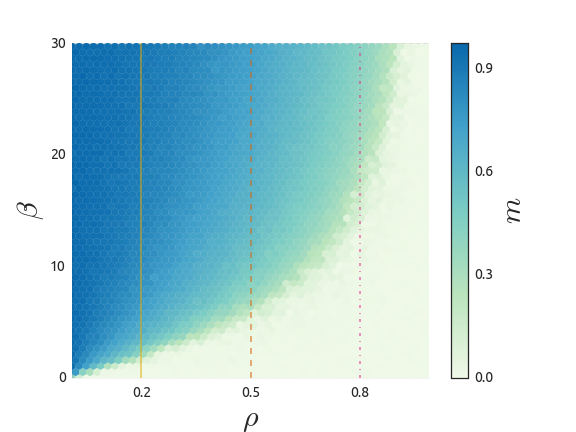
\includegraphics[scale=1.0]{mc-phase-diagram.png}
    \caption{Diagrama de fases do consenso $m$  no plano $\beta \times \rho$, para desconfiança $\ns = 0$.}
\end{figure}
\begin{marginfigure}[-11cm]
    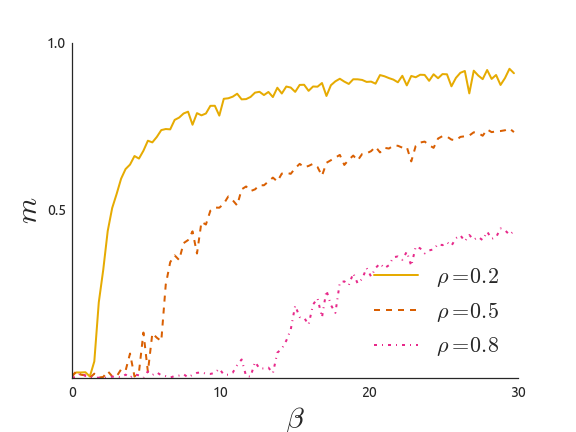
\includegraphics[scale=1.5]{mc-m-curves.png}
    \caption{Curvas de consenso correspondentes às retas verticais na figura \ref{fig:mc-pd-rho}.}
\end{marginfigure}


A diferença que surge na forma da fronteira que delimita as regiões vem do fato que o algoritmo de aprendizado definido por \eqref{eq:Vij}, a saber a função de modulação Bayesiana, é muito mais eficiente do que aquele oriundo da aproximação de campo médio \eqref{eq:V0ij}.
Por diferença na eficiência de um algoritmo de aprendizado entende-se que um número menor de exemplos precisa ser apresentado ao aluno para que ele aprenda a regra do professor.
No contexto de aprendizado social, isso significa que dois parceiros precisam interagir um número menor de vezes para que cheguem a uma opinião comum, e isso se reflete numa pressão crítica menor para que a sociedade atinja o consenso.
Essa é a exata diferença entre as figuras \ref{fig:pd-ferro} e \ref{fig:mc-pd-rho}.

Outra diferença que observamos entre os resultados da simulação de Monte Carlo e o resultado do campo médio é a dependência da pressão crítica com relação ao parâmetro de desconfiança $\ns$.
De fato, na simulação de Monte Carlo, o papel da desconfiança no surgimento de consenso é similar ao estilo cognitivo $\rho$, dificultando o consenso conforme seu valor aumenta.
\begin{figure}[h!]\label{fig:mc-pd-eps}
    \centering    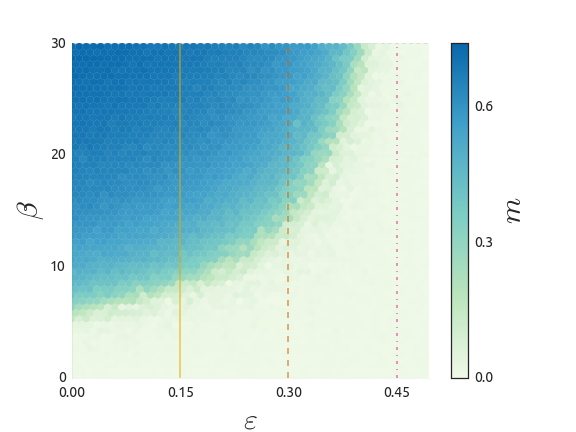
\includegraphics[scale=1.0]{mc-phase-diagram-eps.png}
    \caption{Diagrama de fases do consenso $m$ no plano $\beta \times   \varepsilon$, para desconfiança $\rho = 0.5$.}
\end{figure}
\begin{marginfigure}[-8cm]
    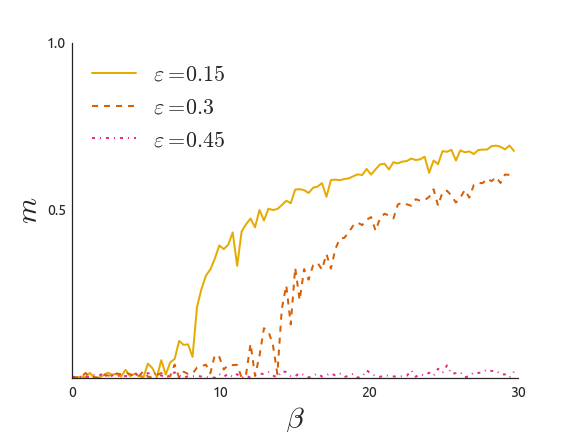
\includegraphics[scale=1.5]{mc-m-curves-eps.png}
    \caption{Curvas de consenso correspondentes às retas verticais na figura \ref{fig:mc-pd-eps}.}
\end{marginfigure}
Essa característica não foi capturada pela aproximação de campo médio, o que explica as diferenças entre as figuras \ref{fig:pd-ferro-eps} e \ref{fig:mc-pd-eps}.
Entretanto, a previsão de que apenas a desconfiança não é capaz de produzir grupos de opiniões distintas é corroborada, devido tamanha similaridade entre $\rho$ e $\ns$ no aparecimento de consenso, o que justifica nossa investida em mecanismos alternativos para tentar entender esse fenômeno.

\subsection{Um Retrato (Estatístico) da Semelhança Entre Agentes}

Outra forma interessante de ver o fenômeno de consenso é através dos histogramas de similaridade $\psi_{ij}$ definida por
\begin{align}
    \psi_{ij} & = \frac{1}{K} \agt{i}\cdot \agt{j} \label{eq:psi-ij}
\end{align}
que nada mais é do que o cosseno do ângulo formado pelos vetores cognitivos dos agentes $i$ e $j$.
De acordo com os diagrama nas figuras \ref{fig:mc-pd-rho} e \ref{fig:mc-pd-eps}, a sociedade tem duas fases, uma desordenada e uma de consenso.
Essas fases são reflexo da distribuição das opiniões a respeito de $\qst$, que estão diretamente relacionadas com $\psi_{ij}$, e portanto devem ser visíveis nos histogramas de similaridade.

\begin{figure}[h!]\label{fig:mc-cons-hist-br}
    \centering
    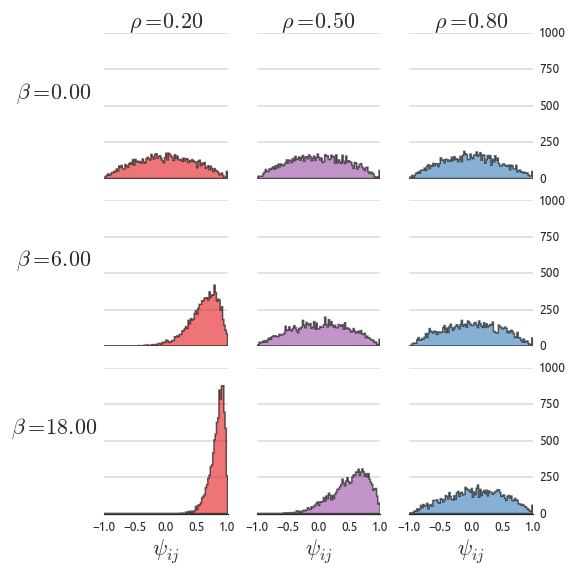
\includegraphics[scale=1.0]{mc-cons-hist-rb.png}
    \caption{Histogramas da similaridade $\psi_{ij}$ para alguns valores do estilo cognitivo $\rho$ e da pressão social $\beta$ com desconfiança $\ns=0$ fixa no modelo para o surgimento de consenso.}
\end{figure}

As figuras \ref{fig:mc-cons-hist-br} e \ref{fig:mc-cons-hist-be} mostram que conforme a pressão social aumenta, e a sociedade caminha para um consenso, a média dos histogramas de semelhança caminha em direção ao valor $1$, e a variância em torno da média vai diminuindo.
A intensidade desse fenômeno está relacionada com os valores do estilo cognitivo $\rho$ e da desconfiança $\ns$, sendo mais perceptível conforme menores seus valores.
Essa característica de baixos valores de $\rho$ estarem associados com uma menor flutuação tolerada nas opiniões é associada com um comportamento conservador, como mostrado em \parencite{Cesar2014,Vicente2014,Caticha2011}.
\begin{figure}[h!]\label{fig:mc-cons-hist-be}
    \centering
    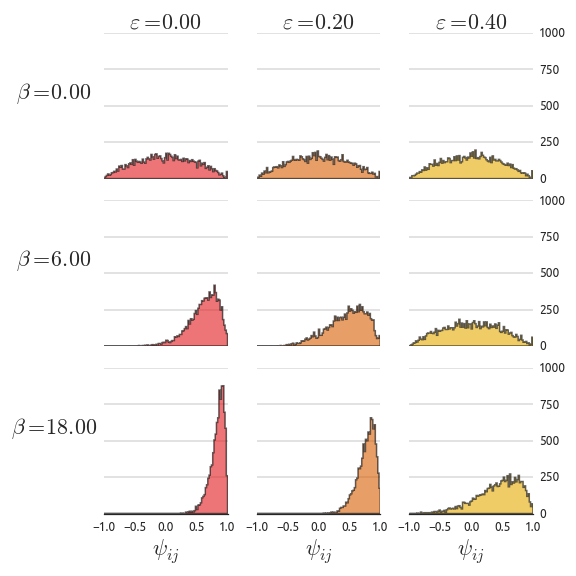
\includegraphics[scale=1.0]{mc-cons-hist-eb.png}
    \caption{Histogramas da similaridade $\psi_{ij}$ para alguns valores da desconfiança $\ns$ e da pressão social $\beta$ com estilo cognitivo $\rho=0.2$ fixo no modelo para o surgimento de consenso.}
\end{figure}

\section{Uma Dinâmica para as Relações Sociais}
\label{sec:DRS}

Um efeito colateral da interação dos agentes, não contemplado pelo modelo acima, é a evolução das relações sociais.
As próximas perguntas que nos fazemos são \emph{``como a escolha de parceiros sociais pode ser feita pelos agentes?''} e \emph{``como essa escolha afeta as fases de desordem e consenso na sociedade?''}.
Para respondê-las, implementaremos um mecanismo de controle das relações baseados nos choques de opinião.
Isso é feito definindo equações para $R_{ij}$ em função das opiniões dos agentes $i$ e $j$.

Restringindo entre $0$ e $1$ os valores de $R_{ij}$, e interpretando o valor nulo como indicativo do agente $i$ não considerar o agente $j$ como parceiro.\footnote{Estamos lidando com um grafo direcionado, representando possíveis não reciprocidades em relações entre agentes.}
A evolução de $R_{ij}$ é dada pela equação \eqref{eq:Rt},
\begin{align}
  R_{ij}(t+1) & = R_{ij} + \lambda\,R_{ij}(1-R_{ij})\sgn\inpr{h_i\,h_j}, \label{eq:Rijt}
\end{align}
fazendo nulo o termo de esquecimento, ou seja $\varphi = 0$.

As relações sociais $R_{ij}$ determinam a probabilidade $p(j|i)$ de cada parceiro $j$ ser escolhido pelo parceiro $i$ nessa rodada.
A escolha mais simples que podemos fazer para relacionar $R_{ij}$ e $p(j|i)$ é a seguinte
\begin{align}
  p(j|i) & = \frac{R_{ij}}{\sum_{k}R_{ik}}, \label{eq:pij-linear}
\end{align}
que pode ser interpretada diretamente como uma medida de distância \footnotemark entre os agentes $i$ e $j$. \footnotetext{na verdade seria o inverso da distância, dado que agentes interagem tem probabilidade nula de interação quando sua relação é também nula.}
A simulação de Monte Carlo é feita de modo análogo ao caso anterior, no qual as relações sociais estavam fixas, com a exceção da escolha do par $(ij)$ ser feita usando a probabilidade $p(j|i)$.

Apenas ajustar a probabilidade de interação entre os agentes não é capaz de produzir polarização de forma consistente.
Com a finalidade de produzir esse efeito, vamos definir a constante de $J_{ij}$, em analogia com o modelo \emph{'antiferromagnético'} usado para o campo médio no capítulo \ref{ch:C2}, mas desta vez como uma função explícita da relações sociais
\begin{align}
    J_{ij} & = \frac{1}{K}\,\sgn\inpr{R_{ij} - \half} \label{eq:Jij-Rij}
\end{align}

Definida dessa maneira, a grandeza $J_{ij}$ direciona o agente $i$ no sentido de aprender a opinião de $j$, caso sua relação esteja \emph{'acima da média'}, ou no sentido de se opor a $j$, caso esteja abaixo.
Por \emph{'acima da média'} entenda que o agente $i$ prefere interagir com $j$ mais do que com outros agentes.

\subsection{Complexidade no Nível das Opiniões}

O primeiro resultado dessa dinâmica pode ser observado através de histogramas da \emph{semelhança}, $\psi_{ij}$ \footnote{definida pela equação \eqref{eq:psi-ij}}.
Para interpretar os histogramas, consideraremos três possíveis situações de equilíbrio da sociedade.

Considere, primeiramente, a situação com baixa ou nula pressão social, $\beta$, indicando que o custo cognitivo da discordância é baixo.
Neste caso, não esperamos que os agentes aprendam as opiniões de seus parceiros e, portanto, nenhum consenso pode ser atingido.
Essa situação é a que ocorre na região clara dos diagramas de fases nas figuras \ref{fig:mc-pd-rho} e \ref{fig:mc-pd-eps}.
Neste caso, os vetores cognitivos dos agentes estarão distribuídos de maneira uniforme na $K$-esfera, e a semelhança entre eles terá média e moda nulas.

Na situação representada pela região escura dos diagramas de fases acima, representando as regiões de consenso, a situação é oposta.
O custo de discordar de um parceiro é elevado, dada a alta pressão social, de modo que os agentes são levados a aprender a opinião uns dos outros.
Isso conduz a uma distribuição de vetores bem mais localizada ao redor do questão $\qst$ ou sua oposta $-\qst$ .
A semelhança entre os agentes terá, portanto, média e moda próximos de $1$, de acordo com os valores do estilo cognitivo $\rho$ e da desconfiança $\ns$.
Esse é o caso em que representa os histogramas nas figuras \ref{fig:mc-cons-hist-br} e \ref{fig:mc-cons-hist-be} da seção anterior.

A terceira situação, que é a novidade desse modelo, é uma em que opiniões opostas em relação à $\qst$ podem coexistir.
É claro que para isso, é necessário uma pressão crítica grande o bastante para que o aprendizado seja necessário, como na situação de consenso.
Entretanto, dada a possibilidade de eliminar relações com agentes que discordam permite que opiniões opostas se mantenham, até que o consenso seja atingido em cada uma delas separadamente de modo que há uma rivalidade global.
Nesse caso, a semelhança entre os agentes também terá média nula, mas apresentará duas modas, cada uma tendendo a $\pm 1$, que indica que uma fração dos agentes compartilha opiniões semelhantes mas opostas a uma outra fração da sociedade.

%% \pagebreak
\begin{figure}[h!]\label{fig:mc-hist-br}
  \centering
  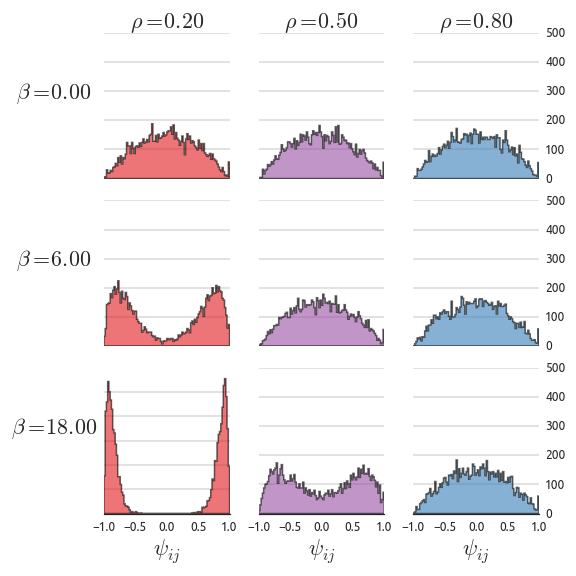
\includegraphics[scale=1.0]{mc-histograms-rhoxbeta.png}
  \caption{Histogramas da similaridade $\psi_{ij}$ para alguns valores do estilo cognitivo $\rho$ e da pressão social $\beta$ com desconfiança $\ns=0$ fixa no modelo com a dinâmica das relações sociais.}
\end{figure}
%% \pagebreak

As três situações acima são ilustrativas e diversos estados intermediários podem surgir, dependendo dos parâmetros que controlam o sistema.
As assinaturas estatísticas dessas situações ajudam, porém, a interpretar as fases da sociedade com relação à dinâmica das relações sociais.

A figura \ref{fig:mc-hist-br} mostra os histogramas de similaridade em diferente condições de estilo cognitivo $\rho$ e pressão social $\beta$, mantendo fixado o valor da desconfiança $\ns=0$.
Note que estilos cognitivos mais conservadores, dados por valores mais baixos de $\rho$, experimentam polarização em condições mais brandas de pressão social e desconfiança.

%% \pagebreak
\begin{figure}[h!]\label{fig:mc-hist-be}
    \centering
    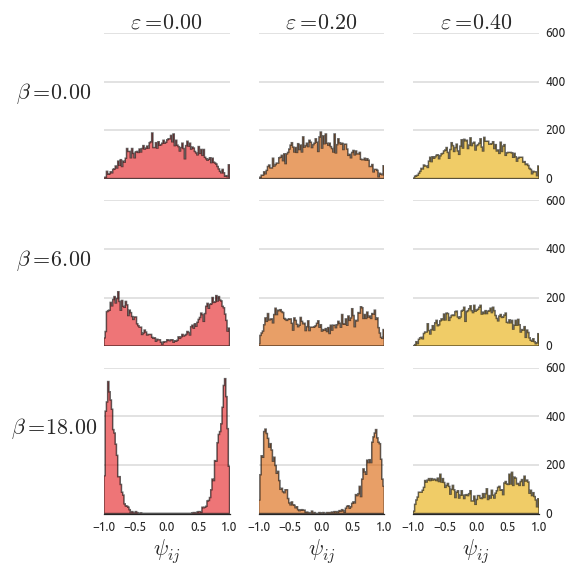
\includegraphics[scale=1.0]{mc-histograms-epsxbeta.png}
    \caption{Histogramas da similaridade $\psi_{ij}$ para alguns valores da desconfiança $\ns$ e da pressão social $\beta$ com estilo cognitivo $\rho=0.2$ fixo no modelo com a dinâmica das relações sociais.}
\end{figure}
%% \pagebreak

A figura \ref{fig:mc-hist-be} mostra histogramas análogos, desta vez em função da desconfiança $\ns$ e da pressão social $\beta$.
Note que a influência da desconfiança sobre o comportamento dos regimes de dissenso, polarização e consenso é similar à do estilo cognitivo, no sentido de dificultar o consenso conforme seu valor aumenta.

É evidente que a distribuição de opiniões com relação a $\qst$ está diretamente relacionada com os histogramas das figuras \ref{fig:mc-hist-br} e \ref{fig:mc-hist-be}.
Com isso podemos concluir que a sociedade tem duas \emph{'regiões de opinião'}, em contraposição à situação de consenso.
Do ponto de vista da teoria de aprendizado de máquina, podemos dizer que uma sociedade polarizada apresenta uma maior complexidade do que no estado de consenso.

\subsection{O Efeito da Dinâmica no Tecido Social}

Outro aspecto dessa complexidade pode ser observada nas matrizes das relações sociais.
Como apontado na seção anterior, as relações sociais formam, inicialmente, um grafo completo, ou seja todos os agentes são parceiros.
Conforme a sociedade evolui, relações podem ser fortalecidas ou destruídas de acordo com a concordância ou discordância dos agentes durante o encontro.

%% \pagebreak
\begin{figure}[h!]\label{fig:mat-br}
    \centering
    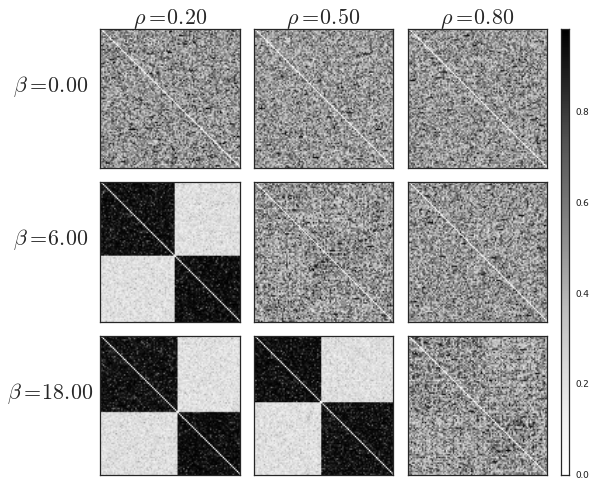
\includegraphics[scale=1.0]{mat-br.png}
    \caption{Matrizes das relações sociais $R_{ij}$ para alguns valores do estilo cognitivo $\rho$ e da pressão social $\beta$ com desconfiança $\ns=0.0$ fixo.}
\end{figure}
%% \pagebreak

Como é possível constatar olhando as figuras \ref{fig:mat-br} e \ref{fig:mc-hist-br}, conforme a distribuição de similaridade se torna mais estreita em relação às modas $\pm1$, estruturas mais evidentes são encontradas nas matrizes de relação social.
Isto é, na situação de polarização é possível observar dois blocos de relações sociais bem definidos, representando agente que interagem mais frequentemente com outros no mesmo bloco do que com agentes do outro bloco.
Essa é a noção de \emph{comunidade} no estudo de redes sociais \footcite{NewmanBook,Reichardt2008}. \footnote{As matrizes apresentadas nas figuras foram analisadas usando o algoritmo de \emph{SPIN} de \parencite{Tsafrir2005}, que reorganizas as linhas e colunas em uma matriz de distâncias de modo que linhas e colunas vizinhas representem menores distâncias.}

Em contraposição à estrutura de comunidade do estado polarizado, podemos observar um grafo completo, dado por uma matriz com um único bloco ou comunidade e relativo ao estado de consenso, ou um grafo aleatório, em que surge nenhuma comunidade e que representa a situação de dissenso nas figuras \ref{fig:mat-br} e \ref{fig:mat-be}.

%% \pagebreak
\begin{figure}[b!]\label{fig:mat-be}
  \centering
  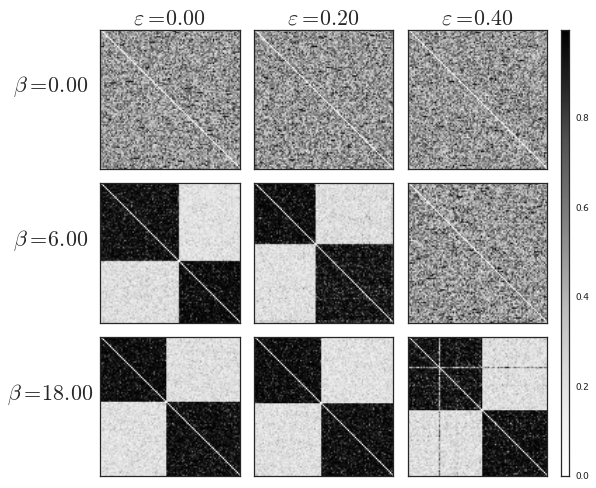
\includegraphics[scale=1.0]{mat-be.png}
  \caption{Matrizes das relações sociais $R_{ij}$ para alguns valores da desconfiança $\ns$ e da pressão social $\beta$ com estilo cognitivo $\rho=0.2$ fixo.}
\end{figure}
%% \pagebreak

Essa complexidade a nível de estrutura social é de uma natureza diferente da complexidade de opiniões.
Embora, por construção, as duas devam estar relacionadas, precisamos de uma forma de garantir que a influência do aprendizado social no estrutura das relações não é coincidência.

\subsection{Outra Forma de Ordem}

Para determinar a influência da opinião dos agentes na estrutura social, vamos introduzir um novo parâmetro de ordem
\begin{align}
    q & = \sum_{(ij)} \sgn\inbk{\inpr{R_{ij}-\half}h_ih_j} \label{eq:q-def}
\end{align}
Para entender como esse parâmetro nos permite associar o estado de polarização às estruturas de comunidade, considere apenas o termo da soma referente aos parceiros $i$ e $j$.

Se a relação $R_{ij}$ entre eles é boa, ou seja\footnote{que faz com que $J_{ij}=\frac{1}{K}$} $R_{ij} > \half$, então eles devem estar na mesma comunidade, e esperamos que a opinião deles tenha o mesmo sinal,  $h_ih_j>0$, no caso em que há polarização na sociedade.
Por outro lado, se eles não estão na mesma comunidade\footnote{fazendo com que $J_{ij}=-\frac{1}{K}$}, $R_{ij}<1/2$, quando há polarização esperamos que os agentes discordem, ou seja $h_ih_j < 0$.
Nesses dois casos, esse termo de $q$ será positivo, pois $\sgn \inbk{\inpr{R_{ij}-\half}h_ih_j}>0$.

Se, em oposição, os agente $i$ e $j$ estão na mesma comunidade mas discordam em opinião, ou concordam em opinião mas estão em comunidades distintas, esse termo será negativo.

O parâmetro $q$, que chamaremos de \emph{medida de estrutura}, é a média sobre todas a relações sociais dessa adequação entre opinião e comunidade, e pode ser vista justamente como um valor de quão bem definidas são as estruturas de comunidade.
Para chegar a essa conclusão basta perceber que o valor de $q$ será mais próximo de $1$ quão melhor for descrever os agentes com mesma opinião como uma comunidade e mais próximo de zero quando essa descrição não for boa.

\begin{figure}[h!]\label{fig:mc-q-curves-rb}
    \centering
    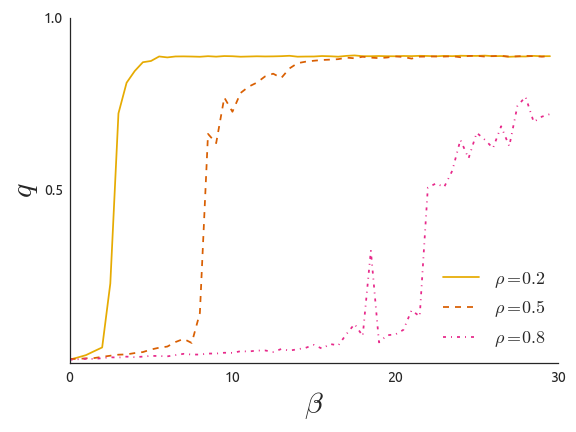
\includegraphics[scale=1.0]{mc-q-curves-rb.png}
    \caption{Curvas da medida de estrutura $q$ em função da pressão social $\beta$ para diferentes valores do estilo cognitivo $\rho$ e com desconfiança $\ns=0$ fixa.}
\end{figure}

As figuras \ref{fig:mc-q-curves-rb} e \ref{fig:mc-q-curves-eb} mostram uma transição entre as fases de desordem e polarização, semelhante à transição de fases na sociedade que atinge consenso.
De modo análogo aos resultados da seção \ref{sec:MCCT}, para valores de pressão social $\beta$ maiores que uma dada pressão crítica, que depende do estilo cognitivo $\rho$ e da desconfiança $\ns$, a sociedade experimenta uma fase em que comunidade de opinião bem formada coexistem.
Abaixo da pressão crítica, porém, não é possível atribuir a multitude de opiniões a comunidades bem estruturadas, e a sociedade vive uma fase de desordem.

\begin{figure}[h!]\label{fig:mc-q-curves-eb}
    \centering
    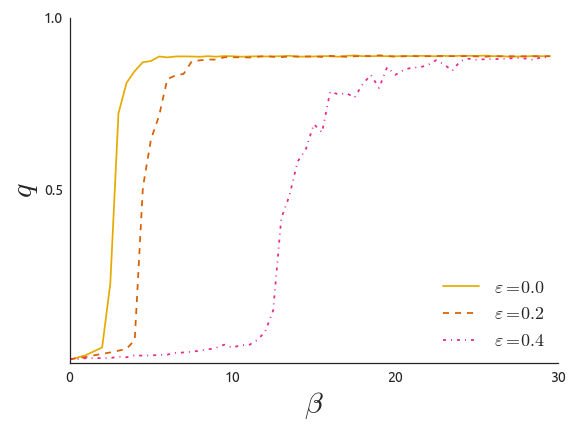
\includegraphics[scale=1.0]{mc-q-curves-eb.png}
    \caption{Curvas da medida de estrutura $q$ em função da pressão social $\beta$ para diferentes valores da desconfiança $\ns$ e com estilo cognitivo $\rho=0.2$ fixo.}
\end{figure}

O efeito do estilo cognitivo e da desconfiança na pressão crítica que possibilita a estruturação de comunidades é análogo ao caso de consenso.
Para valores de $\rho$ maiores, associados a agentes mais liberais, a formação de comunidades exige maior pressão social.
O mesmo pode ser dito sobre os valores de $\ns$.

Podemos ver como essa transição se dá ao longo da evolução da sociedade  tomando como exemplo a figura \ref{fig:mc-q-evol-r}, que mostra o valor de $q$ ao longo das interações entre agentes para alguns valores da pressão social $\beta$ e com $\rho$ e $\ns$ fixos.

\begin{figure}[b!]\label{fig:mc-q-evol-r}
    \centering
    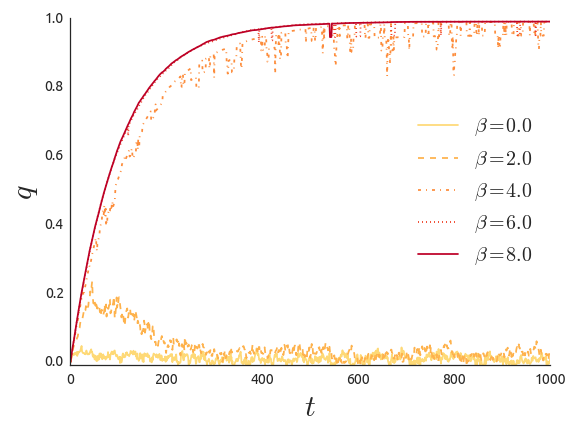
\includegraphics[scale=1.0]{mc-q-evol-r.png}
    \caption{Curvas da medida de estrutura $q$ em função do tempo $t$, em unidades de \emph{número médio de interações por agente}, para diferentes valores da pressão social $\beta$ e com desconfiança $\ns=0$ e com estilo cognitivo $\rho=0.2$ fixos.}
\end{figure}

É possível notar que, para baixos valores de pressão social, os valores de $q$ aumentam por um curto período de tempo, e convergem para zero em seguida.
Para valores mais altos de pressão, a medida de estrutura cresce até convergir para o valor $1$.
Com base na concepção de $q$ como uma medida da estruturação da sociedade, podemos interpretar esse resultado como uma espécie fenômeno que requer uma \emph{'massa crítica'}.
Isso é, as comunidades começam a se formar concomitantes com o aprendizado dos agentes, mas só se estruturam bem se uma porção suficiente de agentes compartilha opiniões mais concentradas.

Com a presente análise, concluímos que as habilidades de escolher o indivíduos com que um agente se relaciona e de escolher a natureza dessa relação são suficientes para criar complexidade social.
Essa complexidade diz respeito tanto à estrutura das relações sociais quanto à distribuição das opiniões e, de fato, é estabelecida como consequência do acoplamento entre as dinâmicas de aprendizado social e da relações entre agentes.
Os resultados apresentados nessa seção são novidade e proporcionam um modelo simples para a formação de estruturas sociais através de um vínculo direto entre a estrutura cognitiva dos agentes e sua interação social.

%% \newpage
\vfill
\pagebreak
\section{Jogos de Partidos}
\label{sec:DM}

Uma vez estabelecida uma dinâmica para as relações sociais que possibilitam o surgimento de grupos com opiniões distintas, podemos nos perguntar como a coexistência desses grupos é afetada por mudanças na pressão social e nas relações entre grupos.
Um  nicho social interessante para estudar a influencia da estrutura e das relações de poder é o das votações parlamentares de um governo democrático.

Com base numa análise, que embora lúdica é bastante interessante, apresentada no \emph{blog} \emph{Todas as Configurações Possíveis} \footcite{MarinoBlog1, MarinoBlog2}, podemos nos perguntar como a mudança de um presidente pode afetar as votações no plenário.
A análise lá apresentada consiste da projeção nas componentes principais da matriz de correlação entre os voto de parlamentares, em várias votações de projetos de lei, ao longo de vários mandatos presidenciais.
O resultado mostra a forte tendencia de partidos como o PMDB em manter seu apoio a projetos da posição, enquanto partidos rivais como PT e PSDB se opõem sistemática e independentemente de quem está no governo.

Nossa ideia é usar a plataforma de aprendizado social e estrutura de comunidade para tentar reproduzir esse comportamento.
Para isso, ao invés de considerar a multitude de partidos políticos no Brasil, lidaremos apenas com três partidos, que vivenciam uma troca de partido no poder ao longo de dois mandatos presidenciais.

\subsection{Um Modelo para a Influência Política}

O cenário é estabelecido com dois \emph{partidos ideológicos} formados por agentes concentrados ao redor de suas respectivas \emph{agendas}, representando os parlamentares de partidos rivais e os quais chamaremos  $A$ e $B$.
Um terceiro partido, ao qual damos o rótulo $C$, sem uma ideologia fixada integra o plenário e participa das votações.
As agendas políticas dos partidos serão denotadas por $\qst_A$ e $\qst_B$.

Sendo rivais, os integrantes dos partidos $A$ e $B$ não procuram uns aos outros para discutir projetos.
Essa situação é bem descrita pela fase de polarização com duas comunidades estudada na seção anterior.
Além disso, esses dois partidos têm ideologias fortes, de modo que eles não aceitam as opiniões dos integrantes do partido $C$ e com isso os integrantes dos partidos $A$ e $B$ discutem apenas entre si.
\begin{figure}[t!]\label{fig:parties-mat}
    \centering
    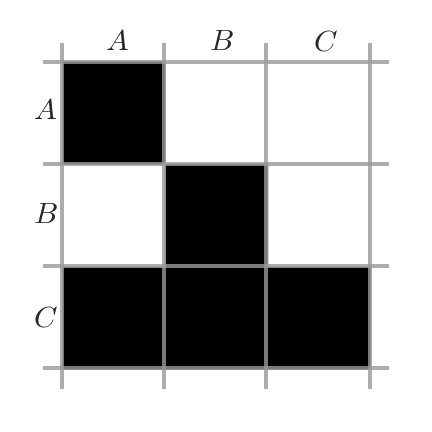
\includegraphics[scale=1.0]{parties-mat.png}
    \caption{Matriz das relações partidárias no modelo com três partidos.}
\end{figure}
O partido $C$, por outro lado, não tem ideologia e se permite interagir com qualquer parlamentar.
Para representar essa estrutura, criamos uma matriz de adjacência, a nível ultra métrico, que representa as possíveis interações entre parlamentares de acordo com seus partidos, ilustrada da figura \ref{fig:parties-mat}

Não estamos, neste momento, preocupados com a formação dos partidos e vamos supor que no período considerado nenhum parlamentar troca de partido, de modo que a estrutura da figura \ref{fig:parties-mat} é fixa.

A dinâmica de aprendizado é similar à usada nos cenários de sociedade com consenso ou polarização, com a exceção de não existir apenas uma questão.
De fato, as agendas política dos partidos $A$ e $B$ representam os projetos propostos por esses partidos e serão, portanto, as questões a serem discutidas pelos agentes.
Vamos convencionar que os parlamentares dos partidos $A$ e $B$ discutem apenas as agendas de seus partidos, enquanto os parlamentares de $C$ escolhem uniformemente entre as duas agendas quando procuram a opinião de outro agente, sendo que quem decide a agenda discutida é o agente que faz o papel de \emph{"professor"}.

Com relação ao estilo cognitivo dos parlamentares, temos que escolher considerar as possíveis diferenças com respeito a políticas liberais ou conservadoras ou considerar os parlamentares com uma mesma orientação nesse sentido.
Esse ponto é delicado e difícil de justificar sem um estudo mais profundo sobre esse aspecto da política brasileira, sendo nenhum de conhecimento do autor.
Por esse motivo, vamos escolher o mais simples, todos os parlamentares são semelhantes em estilo cognitivo.

Em se tratando de política, é certamente um disparate afirmar que não há desconfiança com relação às posições dos parlamentares com relação aos projetos em tramitação.
Entretanto, os resultados que apresentamos até então mostram que o efeito da desconfiança nos regimes da sociedade é similar ao do estilo cognitivo, a saber dificultar o aparecimento de estruturas de ordem.
É com isso em mente que vamos fixar $\ns=0$ nesse modelo, numa forma talvez inadequada de incluir os efeitos da desconfiança no estilo cognitivo\footnote{Outro ponto delicado, mas não completamente sem fundamento.
Para compreender melhor a motivação para isso, basta comparar os gráficos da função de modulação \eqref{eq:f-bayes} para diferentes valores de $\rho$ e $\ns$ e constatar que, com algumas restrições, aumentar $\rho$ é qualitativamente equivalente a reduzir $\ns$ e vice versa, de modo que determinar cada um independentemente não é trivial}.

O papel da pressão social nesse contexto precisa ser revisto.
Lembrando das fases de uma sociedade onde consenso pode surgir, parece natural que dentro de cada partido o valor de $\beta$ deva estar acima da pressão crítica necessária para atingir o consenso.
Porém, não é possível definir de forma heurística o regime no plenário como um todo porque, embora os partidos $A$ e $B$ estejam \emph{'isolados'} e em consenso, o partido $C$ pode mudar de opinião ou, melhor dizendo, posicionamento.
A capacidade de um partido influenciar o outro deve estar relacionada com seu  \emph{'poder político'}.
Vamos então associar o poder político do partido com relação à presidência, ou seja, o partido que estiver no governo deve ter mais poder para pressionar os parlamentares do que aquele que os demais.
Digamos que os poderes políticos do \emph{governo} e da \emph{oposição} são dados por $J_G$ e $J_O$ com $J_G > J_O$.
A \emph{pressão política} será a pressão social efetiva $\beta J_{ij}$, onde
\begin{align}
    J_{ij} & = \begin{cases}
        J_O & \text{se $j$ não faz parte do partido do governo}\\
        J_G & \text{se $j$ faz parte do partido do governo}
\end{cases}
\end{align}

Os partidos  viverão dois mandatos de mesma duração, sendo o primeiro sob o governo do partido $A$ e o segundo sob o governo do partido $B$.
A transição de governo é representada pela troca dos valores de $J_{ij}$.
Para tornar as coisas interessantes, e de certa forma próximas da situação real, vamos assumir que o número de parlamentares do partido $C$ é maior que os dos partidos $A$ e $B$.
A pergunta que queremos responder é: como o partido $C$ se comporta com relação às agendas de $A$ e $B$? Ou, em outras palavras, qual dos partidos rivais recebe o apoio do partido $C$?

Para respondê-la, consideramos duas situações distintas com relação à pressão social $\beta$ no plenário.
Numa delas, a oposição não tem coesão mas o governo tem, ou seja o valor de $\beta$ está abaixo da pressão crítica de modo que a pressão política da oposição não esteja acima da crítica, mas a do governo sim.
Na outra, $\beta$ está acima da pressão crítica, e tanto governo quanto oposição são coerentes, embora o governo exerça uma pressão política muito maior.

\begin{figure}[t!]\label{fig:mc-election-low-b}
    \centering
    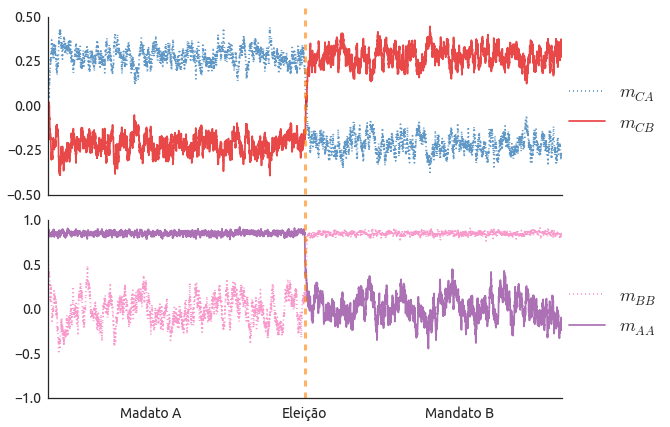
\includegraphics[scale=1.0]{mc-election-low-b.png}
    \caption{Evolução da adesão $m_{rs}$ às agendas $s$ pelo partido $r$ ao longo de dois mandatos com pressão social $\beta=1$ fixo.
    Os parâmetros $J_G=10$ e $J_O=1$ são atribuídos de acordo com o mandato. Os partidos tem tamanho $n_A=n_B=25$ e $n_C=100$ e a eleição ocorre em $t=5000$.}
\end{figure}

A resposta para essa pergunta pode ser obtida olhando para a evolução da \emph{adesão} $m_{rs}$, com $r,s \in \{A,B,C\}$, definida como a média das opiniões dos agentes do partido $r$ sobre a agenda do partido $s$.
Pela construção do modelo, as adesões interessantes serão $m_{CA}$, $m_{CB}$, $m_{AA}$ e $m_{BB}$, pois queremos saber o posicionamento do partido $C$ e devemos monitorar os outros partidos para saber como se comportam com relação às próprias agendas.

\begin{figure}[t!]\label{fig:mc-election-high-b}
    \centering
    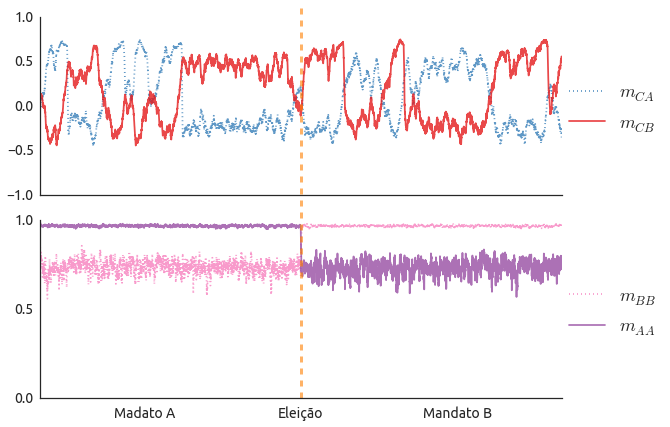
\includegraphics[scale=1.0]{mc-election-high-b.png}
    \caption{Evolução da adesão $m_{rs}$ às agendas $s$ pelo partido $r$ ao longo de dois mandatos com pressão social $\beta=5$ fixo.
Os parâmetros $J_G=50$ e $J_O=1$ são atribuídos de acordo com o mandato. Os partidos tem tamanho $n_A=n_B=25$ e $n_C=100$ e a eleição ocorre em $t=5000$.}
\end{figure}

A figura \ref{fig:mc-election-low-b}, quando a pressão social está abaixo da pressão crítica, mostra que, embora o partido $B$ comece concentrado, a falta de coesão faz com que se desprenda da sua agenda e o mesmo ocorre quando $A$ deixa de ser governo e passa a ser oposição.
Nesse caso, não temos partidos ideológico ao longo dos dois mandatos.
Por conta disso, o partido $C$ acaba apoiando o governo, seja do partido $A$ ou do partido $B$.

No caso de pressão acima da pressão crítica, ilustrada na figura \ref{fig:mc-election-high-b}, é possível perceber que os partidos rivais $A$ e $B$ continuam focados em suas agendas, embora sofram um pequeno abalo no valor absoluto do consenso quando não estão no governo.
Por outro lado, a adesão do partido $C$ oscila entre governo e oposição, de modo que seu apoio não é tão óbvio quanto no caso da pressão abaixo da crítica.
Esse resultado é sensível ao tamanho relativo dos partidos e da relação de poder entre governo e oposição, podendo não ser observado caso a diferença de poder não seja muito grande ou caso os partidos sejam distribuídos de forma mais justa ou com a maioria em um dos partidos ideológicos.
Todavia, esse resultado reproduz parte do comportamento observado nos deputados em votações ao longo dos mandatos dos ex-presidentes \emph{Fernando Henrique Cardoso} e \emph{Luiz Inácio Lula da Silva}, como veremos a seguir.
Embora a confirmação experimental ainda não seja possível, podemos ter uma ideia de quais elementos do modelo providenciam uma explicação qualitativa do comportamento político no congresso nacional.

\subsection{Uma Análise das Votações em Plenário ou\\
            `A Valsa dos Partidos` no Brasil}

%% inserir análise experimental

Como mencionado na seção anterior, a análise dos resultados de votações em plenário ao longo dos mandatos presidenciais realizada por \emph{R. Marino} em seu \emph{`blog`} inspirou a elaboração do modelo de agentes apresentado acima.
A aquisição dos dados foi feita através das páginas mantidas pelos parlamentares ou através de requerimento direto à assessoria da câmara.

Esses dados consistem das informações sobre o projeto de lei sendo votado, o dia da votação, além do nome, do voto, do partido de filiação e do estado de cada parlamentar votante.
A análise presente em \parencite{MarinoBlog1, MarinoBlog2} consiste na visualização da evolução na projeção de duas componentes principais da matriz de correlação desses votos, identificados pelos partidos.
Felizmente, os dados estão acessíveis nestes sítios.

O que fizemos foi pegar os dados disponíveis e identificar a concordância média entre os votos do \emph{PMDB} e do \emph{PSDB} e entre os votos do \emph{PMDB} e do \emph{PT}, bem como a coesão entre os votos do \emph{PT} e \emph{PSDB}, ao longo dos dois mandatos do \emph{FHC} e dos dois mandatos do \emph{Lula}.
Embora a concordância entre dois deputados em relação à um dado projeto de lei não seja idêntico ao que foi chamado de adesão, $m_{rs}$, na elaboração do modelo, é evidente que estão diretamente relacionadas, de modo que trataremos a concordância como se fosse a adesão.

Note, porém, que não temos como determinar a pressão social à qual a câmara estaria submetida ou a influência política do partido no governo.
Podemos, no máximo, comparar os dados com os cenários ilustrados pelo modelo e ver quais características do modelo podem fazer algum sentido.
\begin{figure}[t!]\label{fig:dados-marino}
    \centering
    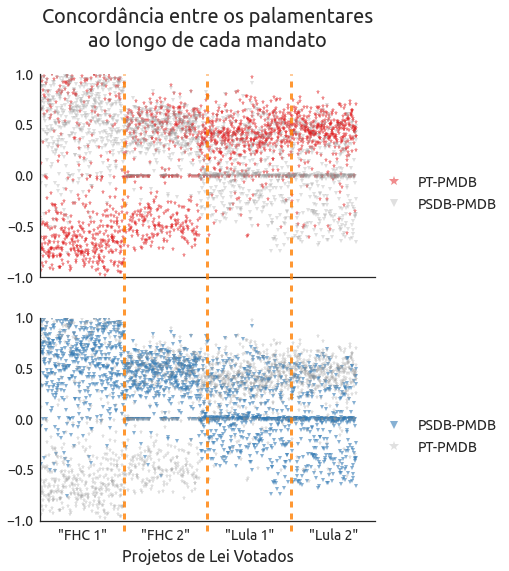
\includegraphics[scale=1.0]{dados-marino.png}
    \caption{Evolução da concordância nos votos em câmara dos deputados do \emph{PMDB} com os deputados do \emph{PSDB} ou \emph{PT} ao longo dos mandatos de \emph{FHC} e \emph{Lula}.}
\end{figure}

A figura \ref{fig:dados-marino} mostra a mudança no comportamento da concordância entre os deputados do \emph{PMDB} com os partidos no poder ou na oposição. \footnote{Os resultados apresentados nessa seção, diferente da análise feita em \parencite{MarinoBlog1}, não fez uso de nenhum pré-processamento dos dados.}
É possível notar que o apoio do \emph{PMDB} está sempre mais concentrado no partido que está na presidência, mudando de forma quase abrupta na transição de governo que se deu entre \emph{FHC} e \emph{Lula}.
Nesse gráfico, cada ponto é a média da concordância entre todos os deputados do \emph{PMDB} com todos aqueles do \emph{PSDB} (em azul) ou do \emph{PT} (em vermelho) para um dado projeto de lei em votação, ordenados pela data.
\begin{figure}[t!]\label{fig:dados-marino-medias}
    \centering
    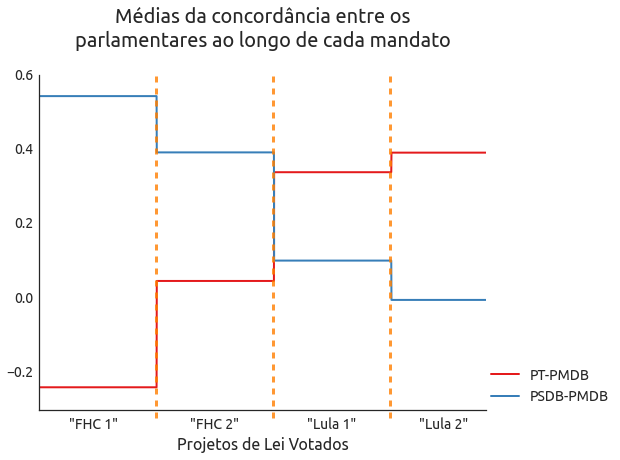
\includegraphics[scale=1.0]{dados-marino-medias.png}
    \caption{Evolução da média das concordância nos votos em câmara dos deputados do \emph{PMDB} com os deputados do \emph{PSDB} ou \emph{PT} ao longo dos mandatos de \emph{FHC} e \emph{Lula}.
Essa figura ilustra o apoio médio do \emph{PMDB} em cada mandato considerado.}
\end{figure}

A figura \ref{fig:dados-marino-medias} facilita a visualização substituindo cada ponto pela média sobre o mandato.
Embora a média não seja um bom representativo, dado que somente o número de projetos de lei apoiados não representa completamente as conquistas políticas \footnote{Alguns projetos podem ser mais importantes que outros na realização da agenda política de cada partido, então se um partido consegue o apoio necessário em projetos importantes, mesmo que em menor número, pode não estar de fato sofrendo uma oposição.}, o comportamento da média no segundo mandato do \emph{FHC} e no primeiro do \emph{Lula} exibem o mesmo comportamento do modelo no cenário de pressão abaixo da crítica.
Isso pode indicar qual a influência política do partido no governo é mais relevante do que a pressão política na câmara em si.

Entretanto, ao verificarmos a evolução da coesão interna do partidos \emph{`rivais`}, \emph{PSDB} e \emph{PT}, percebemos que nenhum dos cenários estabelecidos pelo modelo explica bem o comportamento observado nos dados.
Como visto na figura \ref{fig:dados-marino-coesao}, tanto \emph{PT} quanto \emph{PSDB} passam por um enfraquecimento na coesão ao longo dos quatro mandatos considerados.
\begin{figure}[t!]\label{fig:dados-marino-coesao}
    \centering
    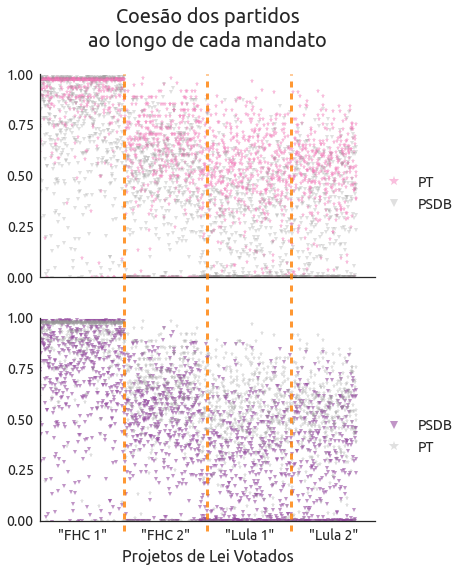
\includegraphics[scale=1.0]{dados-marino-coesao.png}
    \caption{Evolução da coesão interna do \emph{PSDB} ou \emph{PT}, observada através dos votos dos deputados em câmara, ao longo dos mandatos de \emph{FHC} e \emph{Lula}.}
\end{figure}

Novamente, é mais fácil olhar apenas para a média sobre cada mandato para visualizar mais facilmente esse comportamento, que é completamente distinto do produzido pelo modelo.
Isso nos diz que o modelo faz hipóteses inadequadas sobre algum aspecto do comportamento político, e precisa ser refinado de alguma forma.
Embora mais estudo nessa direção seja necessário, o autor acredita que as hipóteses que devam ser atacadas sejam a de isolamento do partidos rivais e a natureza estática da agenda de cada partido, embora a imposição de um único estilo cognitivo a todos os agentes, independente do partido, possivelmente tenha uma influência notável.
\begin{figure}[t!]\label{fig:dados-marino-coesao-medias}
    \centering
    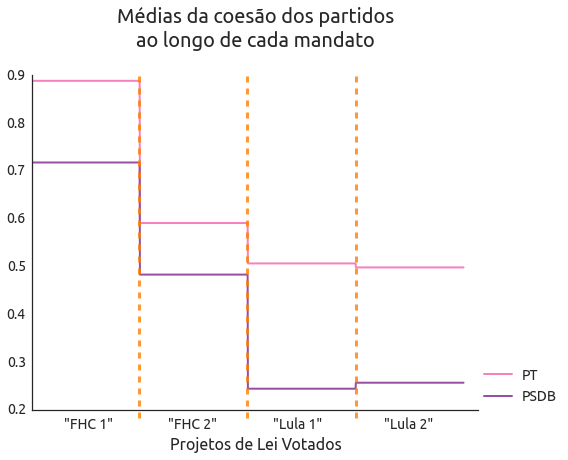
\includegraphics[scale=1.0]{dados-marino-coesao-medias.png}
    \caption{Evolução da média da coesão interna do \emph{PSDB} ou \emph{PT}, observada através dos votos dos deputados em câmara, ao longo dos mandatos de \emph{FHC} e \emph{Lula}.}
\end{figure}

Com base nos dados apresentados, podemos concluir que o modelo de formação de opinião através da interação de agentes reproduz parte do comportamento político observado no plenário brasileiro.
Entretanto, a formação de coalizões, não tendo sido extensivamente estudada, talvez possa explicar as disparidade entre o modelo e a realidade.
Dito isso, o fato do modelo reproduzir algum comportamento observado é em si impressionante e nos proporciona uma base qualitativa de interpretação dos processos políticos, e talvez estejamos um passo mais perto da capacidade de compreendê-los o suficiente para fazer previsões.

Para finalizar, um comentário especulativo sobre os dados sobre o apoio do \emph{PMDB} e as eleições presidenciais.
Notem que do primeiro para o segundo governo \emph{FHC}, o \emph{PSDB} experimentou uma redução no apoio recebido pelo \emph{PMDB}.
Situação oposta à do \emph{PT} entre o primeiro e segundo mandatos do \emph{Lula}.
Dado que o \emph{PSDB} perdeu a eleição presidencial após o segundo governo \emph{FHC} e que o \emph{PT} ganhou a eleição presidencial após o segundo governo \emph{Lula}, será que é sensato questionar se há uma relação entre a capacidade de manter o poder e o apoio de partidos \emph{`maleáveis`}?
A capacidade de responder essa pergunta está além do que podemos fazer por enquanto, dada a juventude da democracia brasileira pós ditadura militar, mas fazer perguntas tolas são sempre uma boa maneira de incentivar uma investigação mais profunda.

% Neste capítulo concluímos que o mecanismo de formação de estrutura social proposto é capaz de introduzir complexidade nas relações sociais e na distribuição de opiniões.
% Vimos um exemplo de como fenômenos sociais, no caso as disputas políticas na câmara, podem ser possivelmente descritos através de um modelo preocupado em relacionar as características cognitivas aos fenômenos sociais\footnote{note que embora tenha sido apresentado de forma um tanto lúdica, o modelo para as votações em plenário acabou se mostrando impressionante em vários aspectos.}.
